\section{Integrationstest}
\subsection{Test med spændingsdeler}
For at teste spændingsdeleren på fumlebrættet har vi brugt Waveforms til at generere to signaler, et sinussignal med en masse forskellige
frekvenser, og et DC signal med 2 V.  Vi har indsendt signaler med frekvenser mellem 10 Hz og 500 Hz og her kan det ses, at signalet dæmpes når frekvensen stiger. 



\subsection{Test med vandsøjle}
Integrationstest
Transducer med forskellige tryk
Formålet med testen er at undersøge hvilke output de forskellige tryk på vandsøjlen giver, samt at se om der er en sammenhæng mellem tryk og spænding.

Der blev udført en række test, hvor hele systemet var koblet sammen. Hvor vi undersøgte hvilke spændinger vores system ville give ved et tryk på 100 mmHg, 50 mmHg og 10 mmHg.  Fra WaveForms gav vi subtraktoren 2 V, og resten af systemet fik +5 og -5 V. I intergretionstesten ville vi forvente at vores spændinger ville ligger inden for et interval der hedder + 2 og - 2 V, da subtraktoren nedsænker signalet med 2V.

Resultatet af testen blev:

\vspace{0.2 cm}

\textbf{100 mmHg  =  -0,370 V:}

\vspace{0.2 cm}

\begin{figure}[h!]
	\centering
	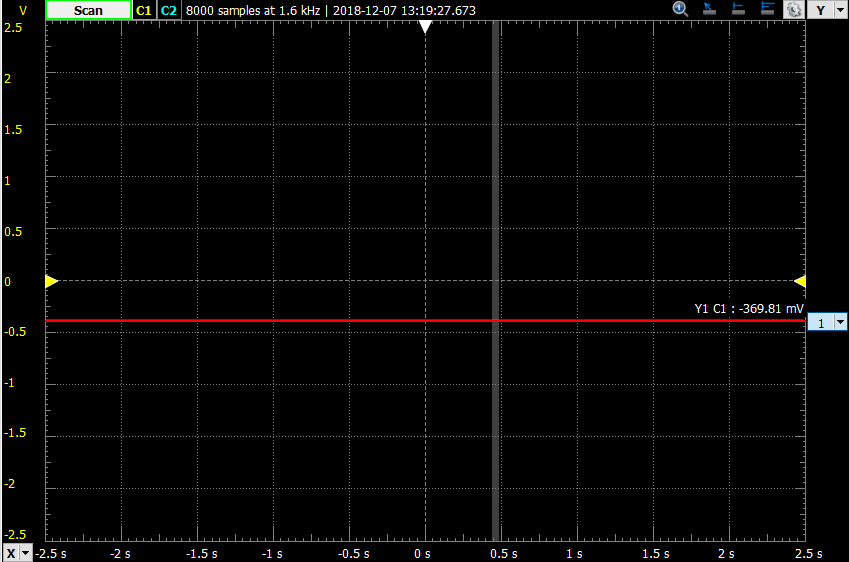
\includegraphics[width=1\linewidth]{Hardwaredesign/mmHg100}
	\caption{Spændning ved 100 mmHg tryk}
	\label{fig:100mmHg}
\end{figure}

\vspace{0.2 cm}

\textbf{50 mmHg  =  -1,173 V:}

\vspace{0.2 cm}

\begin{figure}[h!]
	\centering
	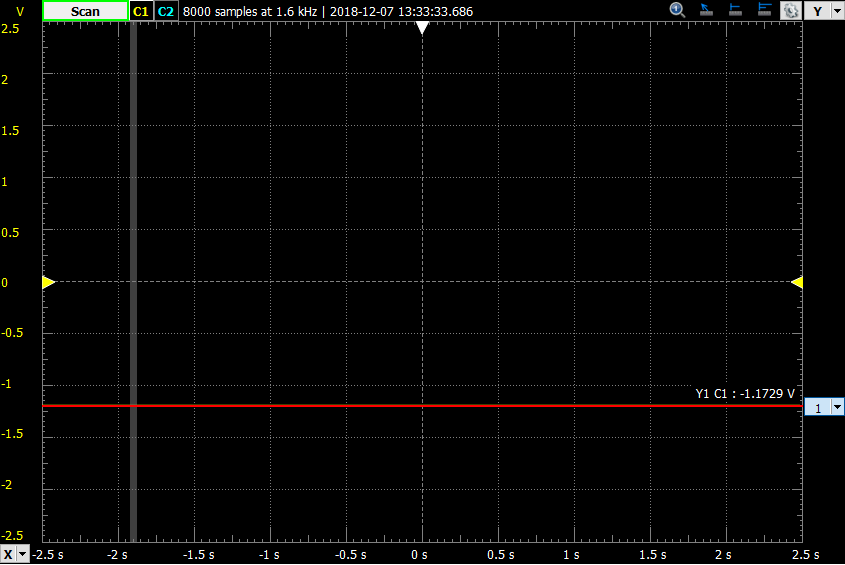
\includegraphics[width=1\linewidth]{Hardwaredesign/mmHg50}
	\caption{Spændning ved 50 mmHg tryk}
	\label{fig:50mmHg}
\end{figure}

\vspace{0.2 cm}

\textbf{10 mmHg  =  -1,804 V:}

\vspace{0.2 cm}

\begin{figure}[h!]
	\centering
	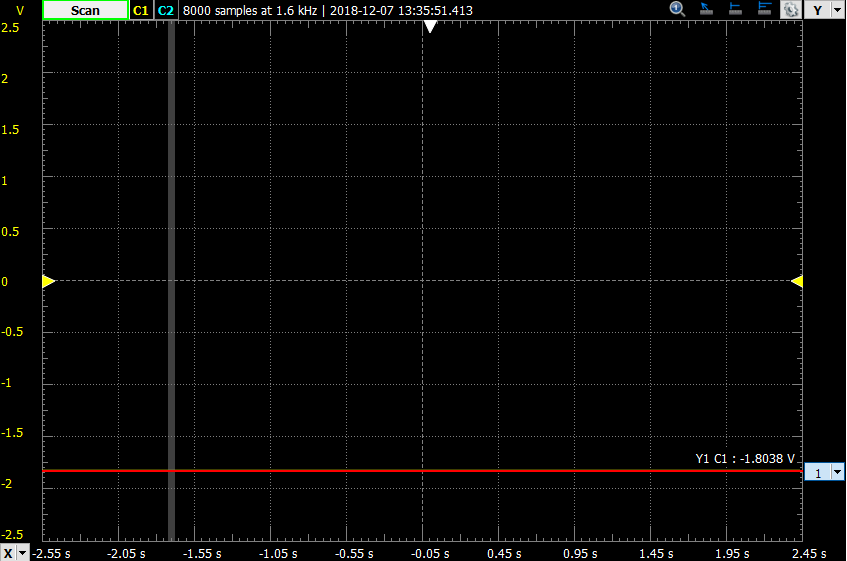
\includegraphics[width=1\linewidth]{Hardwaredesign/mmHg10}
	\caption{Spændning ved 10 mmHg tryk}
	\label{fig:10mmHg}
\end{figure}

\vspace{0.2 cm}

\textbf{0 mmHg  =  -1.966 V:}

\vspace{0.2 cm}


\begin{figure}[h!]
	\centering
	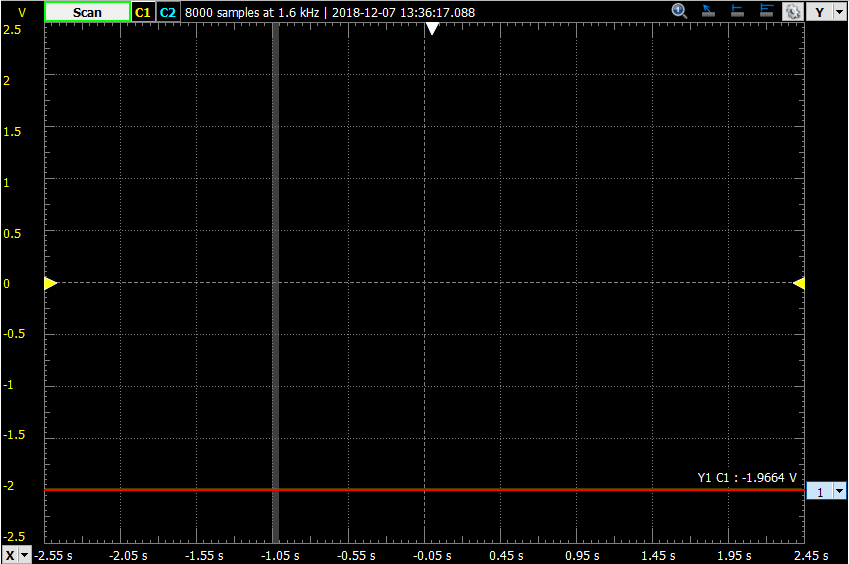
\includegraphics[width=1\linewidth]{Hardwaredesign/mmHg0}
	\caption{Spændning ved 0 mmHg tryk}
	\label{fig:0mmHg}
\end{figure}

\vspace{0.2 cm}

\textbf{Andre tryk:}

\vspace{0.2 cm}

Vi ved at vandsøjlen er 1360 mm høj ved et tryk på 100 mmHg. Denne information kunne vi benytte til at udregne nogle andre tryk ved at ændre på vandhøjden i søjlen.
Der ønskes at undersøge trykket for 25 mmHg og 75 mmHg, hvilket er beregnet på følgende måde:

1360 * 0,25 = 340 mm
1360 * 0,75 = 1020,0 mm

Vi tilsluttede transduceren til vandsøjlen, og påfyldte vand i søjlen til de beregnede højder.
\newpage

\textbf{25 mmHg  =  -1.5744 V:}

\begin{figure}[h!]
	\centering
	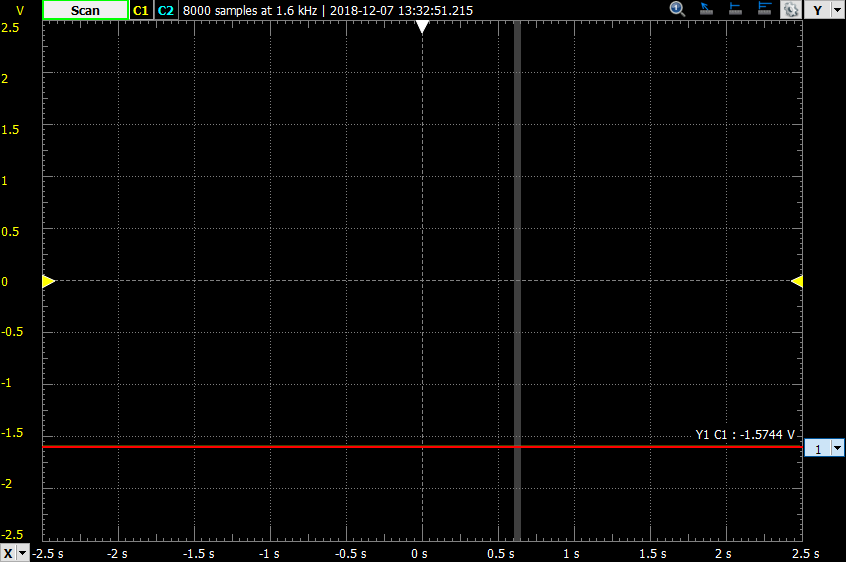
\includegraphics[width=1\linewidth]{Hardwaredesign/mmHg25}
	\caption{Spændning ved 25 mmHg tryk}
	\label{fig:mmHg25}
\end{figure}

\textbf{75 mmHg  =  -0.771 V:}

\begin{figure}[h!]
	\centering
	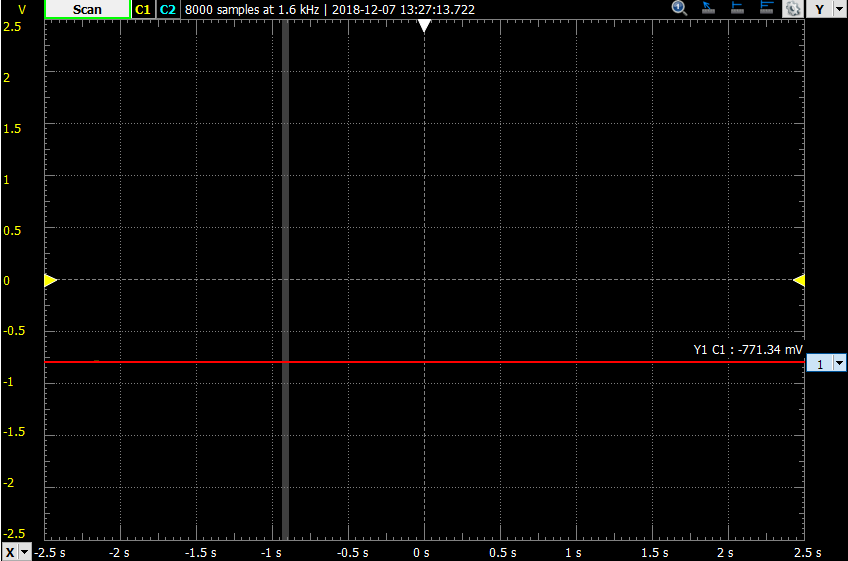
\includegraphics[width=1\linewidth]{Hardwaredesign/mmHg75}
	\caption{Spændning ved 75 mmHg tryk}
	\label{fig:75mmHg}
\end{figure}
\newpage
Tager vi alle vores målinger og plotter dem, ses der en tydelig sammenhæng mellem tryk og spænding.

\vspace{0.2 cm}

\textbf{Plot af spændningerne:}

\vspace{0.2 cm}

\begin{figure}[h!]
	\centering
	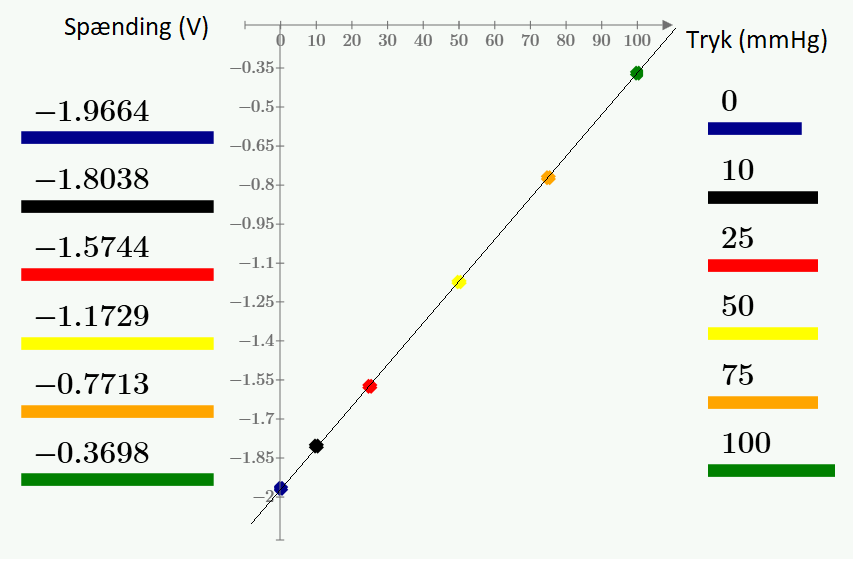
\includegraphics[width=1\linewidth]{Hardwaredesign/trykgraf}
	\caption{Spændning som funktion af tryk}
	\label{fig:trykgraf}
\end{figure}

Testen gik som forventet.


